\documentclass{article}

\usepackage{../swiftnav}
\usepackage{../swiftnav_tikz}

\usepackage{draftwatermark}
\SetWatermarkLightness{0.85}
\SetWatermarkText{Preliminary}
\SetWatermarkScale{4}

% ---------------------------------------------------------------------------

\version{1.0}
\title{SwiftGNSS Datasheet}
\author{Swift Navigation}
\date{\today}

\begin{document}

\maketitle

%\begin{center}
%\resizebox{\linewidth}{!}{\textbf{\color{alt}SwiftGNSS Datasheet}}
%\end{center}
%\vspace{10pt}

\begin{multicols*}{2}
\raggedcolumns


\section*{Features}
\large
\label{sec:Features}
\begin{itemize}
  \bulletnoindent
  \item Item 1.
  \item Item 2.
  \item Item 3.
\end{itemize}
\normalsize

\section*{Applications}
\large
\label{sec:Applications}
\begin{itemize}
  \bulletnoindent
  \item Item 1.
  \item Item 2.
  \item Item 3.
\end{itemize}
\normalsize

\section*{Description}

\lipsum[1-3]

\begin{center}
  % The block diagram code is probably more verbose than necessary
  \begin{tikzpicture}[auto, node distance=1.5cm,>=latex']
    % We start by placing the blocks
    \node [input, name=input] {};
    \node [sum, right of=input] (predictsum) {$\scriptscriptstyle +$};
    \node [block, right of=predictsum] (C) {$\frac{\omega_{n}^{2}}{k}$};
    \node [sum, right of=C] (vpredictsum) {$\scriptscriptstyle +$};
    \node [block, right of=vpredictsum] (int) {$\frac{1}{s}$};
    \node [block, right of=int] (secint) {$\frac{1}{s}$};
    \node [output, right of=secint] (output) {};
    \draw [->] (input) -- node[name=u] {$\theta (u)$} (predictsum);
    \draw [->] (predictsum) -- node[name=e] {$e_{\hat{\theta}}$} (C);
    \draw [->] (C) -- node[coordinate, name=meas] {} (vpredictsum);
    \draw [->] (vpredictsum) -- node[name=ve] {$e_{\hat{\dot{\theta}}}$} (int);
    \draw [->] (int) -- node[name=ydot, below] {$\hat{\dot{\theta}}$} (secint);
    \draw [->] (secint) -- node[name=y] {$\hat{\theta}$} (output);
    \node [block, above of=int, node distance=1cm] (D) {$2 \zeta \omega_{n}$};
    \draw [->] (ydot) |- (D) -| node [name=negfb,pos=0.98] {$-$} (vpredictsum);
    \coordinate [below of=secint, node distance=1cm] (ydown);
    \draw [->] (y) |- (ydown) -| node [name=negfb,pos=0.98] {$-$} (predictsum);
  \end{tikzpicture}
  \captionof{figure}[ToC entry]{A block diagram of the existing delay-locked loop.}
\end{center}

\lipsum[5-6]

\end{multicols*} 

\section*{Electrical Specifications}

\begin{center}
  \begin{threeparttable}[b]
    \begin{tabular}{llrrrr}
      \toprule
      Symbol & Parameter & Min & Typ. & Max & Unit \\
      \midrule
      $V+$ & Supply voltage & 3.5 & & 5.5 & V \\
      $I_{in}$ & Supply current & & 150\tnote{(1)} & 550 & mA \\
      $I_{out}$ & Current draw from 3.3V output & & & 222 & mA \\
      $T$ & Operating temperature & -40 & & 55 & $^\circ$C \\
      $Z_{ant}$ & Antenna input impedance &  & 50 & & $\Omega$ \\
      \bottomrule
    \end{tabular}
    \begin{tablenotes}
    \item [1] Depending on the firmware configuration.
    \end{tablenotes}
  \end{threeparttable}
\end{center}

\begin{multicols}{2}

\noindent
Supply voltage \dotfill 5.5 V \\
Supply current \dotfill 550 mA \\
Current draw from 3.3V output \dotfill 222 mA \\
Operating temperature \dotfill -40 -- 55 $^\circ$C \\
Antenna input impedance \dotfill 50 $\Omega$

\noindent
Supply voltage \dotfill 5.5 V \\
Supply current \dotfill 550 mA \\
Current draw from 3.3V output \dotfill 222 mA \\
Operating temperature \dotfill -40 -- 55 $^\circ$C \\
Antenna input impedance \dotfill 50 $\Omega$

\end{multicols}

\section*{Mechanical Specifications}
\begin{figure}[h]
  \centering
  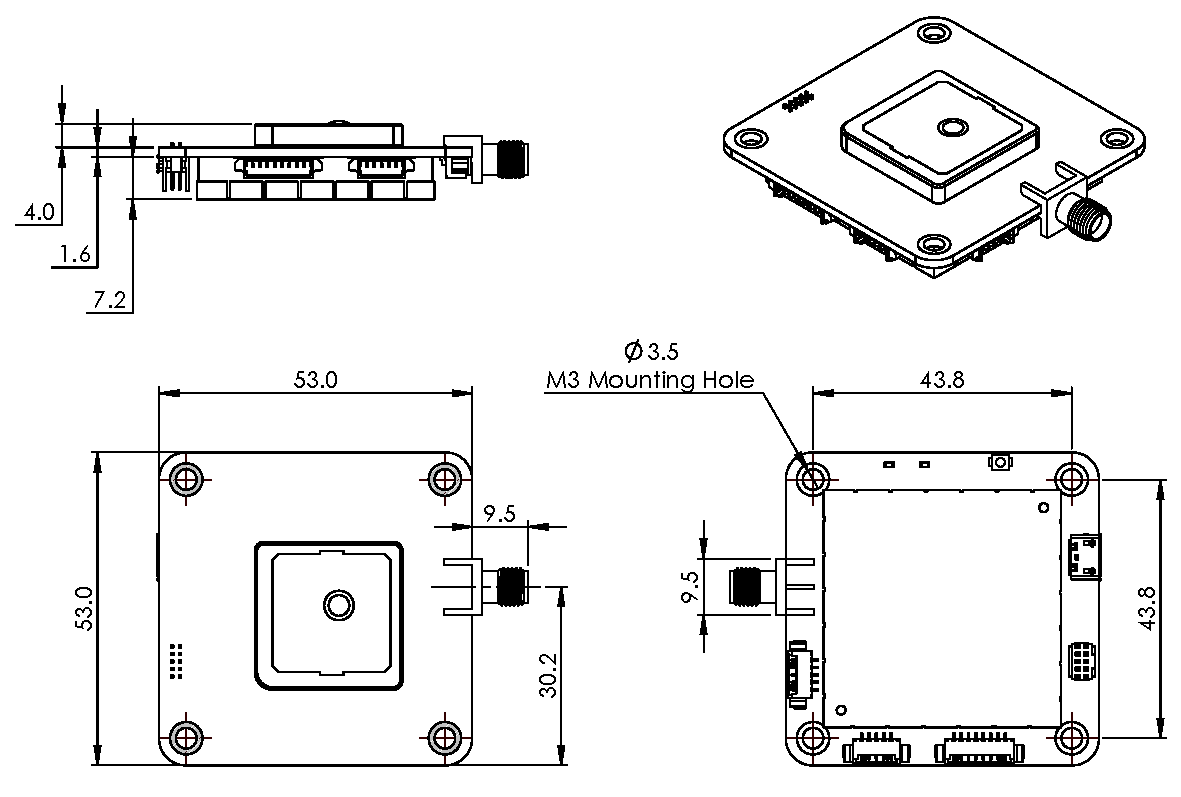
\includegraphics[scale=0.75]{swiftnav_v2_2_mechanical.pdf}
\end{figure}

All dimensions are in millimeters. Drawing not to scale.

3D CAD models are available from our website, \url{http://www.swift-nav.com}.

\end{document} 
